\documentclass[10pt]{article}
\usepackage{geometry}
\geometry{
 	a4paper,
 	total={170mm,257mm},
 	left=15mm,
 	top=10mm,
 }
\usepackage{amsmath,amsthm,amssymb,amsfonts,listings,graphicx,caption,subcaption,hyperref,mathtools, multicol, booktabs}
\newtheorem{theorem}{Theorem}
\begin{document}
\title{Factor large numbers with parallelization}
\author{names...}
\maketitle

\section{Background}
Being able to securely transer information is critial to communications, we rely on it everytime we go on internet where we want the information we send not to exposed to others. And this is made possible by encoding and deconding the message -- suppose you want to send your account information to your bank, a \textit{key pair} contains \textit{public key} and \textit{private key} will be created, another keypair will also be created in the bank,
\begin{equation*}
\text{User} 
\begin{cases}
\text{public key 1}\\
\text{private key 1}            
\end{cases}\qquad \rightleftharpoons \qquad
\text{Bank} 
\begin{cases}
\text{public key 2}\\
\text{private key 2} 
\end{cases}
\end{equation*}
you and bank will both make the public key open to everyone, so you can encode the message you want to send to the bank by using public key 2, and you know the only one can decode it is the bank with their private key 2. You will also encode your message with your private key 1 so that the bank will know it is truly you who sends the message by decoding it using your public key 1. \\
\-\ \\
The encoding and decoding is done by using an algorithm called RSA, where it relies on the fact that it is extremely difficult to factor a large number to two prime numbers. We will first introduce a simple algorithm that is used to do prime factorization -- Pollard's $p-1$ Algorithm, and we will build a parallel version of this algorithm to see how much faster we can gain from the parallelization with a comparison to sequential implementation, then we will introduce a more sophisticate algorithm -- Pollard Rho.  

\section{Euler-Fermat and Factoring}  
We will use the theorem of Fermat's little theorem(a special case of Euler-Fermat) to help us find the two prime factors of a given number, first we state an equivalent theorem\cite{fermat}, 
\begin{theorem}
If $p$ is a prime number, then for any integer $a$, if $a$ is not divisible by $p$, the number $a^{p-1}-1$ is an integer multiple of $p$, i.e.  
\[a^{p-1} \equiv 1 \enspace (\text{mod}\enspace p)\]
\end{theorem}
\noindent Now suppose we have an integer $N = pq$ where $p$ and $q$ are prime, and from theorem 1 we have $a^{p-1} \equiv 1 \enspace (\text{mod}\enspace p)$ for $a$ coprime with $p$, or equivalently $a^{p-1}=k_1p+1$ for some integer $k_1$,\\
Let $L$ be an integer multiple of $p-1$ i.e. $L=k_2(p-1)$, then we have: 
\begin{equation*}
a^L=(a^{p-1})^{k_2}=(k_1p+1)^{k_2}=\binom{k}{0}1 + \binom{n}{1}(k_1p) + \cdots +
\binom{n}{n}(k_1p)^{k_2}
\end{equation*}
so $a^L-1$ is also a multiple of $p$, that is $a^L \equiv 1 \enspace(mod\enspace p)$.\\
Thus, greatest command divisor $gcd(a^L-1, N)=p$ (for non-trivial solution e.g. 1 or N), so this gives us a way to find $p$(and $q$) if given $N=pq$, however, the problem is that we need to have $a^L-1$ to do the calculation, and we do not know $p$ yet how do we obtain $L$? We introduce \textit{Pollard's $p-1$ algorithm}.
\subsection{Pollard's $p-1$ algorithm\cite{suzuki}}
We first start by 1) choosing a number $a$ that is coprime to $N$, then we want to find a good integer $L=k_2(p-1)$, we do this by iterating over possible product of $k_2$ and $(p-1)$, more concretely, 2) let $L= k!$ with $k$ iterate over $[1, 2, \cdots, \text{some large integer}]$, thus there is a good chance $L=k!=K_1K_2$ will be equal to $(p-1)k_2$ at some point of the iteration. Finally, we obtain $p$ by 3) compute $gcd(a^L-1, N)$, if the result is $1$ or $N$ then iterate to next $k$ in step 2).\\
\-\ \\
We show this by going through a real example,\\
\-\ \\
\underline{Example:} Factor 119\\
\begin{align*}
1)& \quad \text{since 119 is odd, let us choose $a=2$}\\
2)& \quad L=k!, \text{first we choose $k=2$ so $L=2$}\\
3)& \quad \text{compute gcd: }\quad gcd(2^2-1, 119) = gcd(3,119) = gcd(2,3) = 1\\
&\quad \text{this is a trivial solution, we change $k$ to $4$ in step 2)}\\
&\quad 2) \quad L = 3! = 6\\
&\quad 3) \quad gcd(2^6-1, 119)=gcd(63, 119)=gcd(56,63)=gcd(7,56)=7
\end{align*}
so we have $p=7$, this is correct as we used $7\times17$ to create the 119 in this example.\\
In the follwing sections we will discuss this algorithm's sequential and parallel implementation in Python. 
\subsection{Sequential implementation}
the pseudo-code is straight froward according to example above, see complete code in appendix A.1.
\begin{verbatim}
Choose int a coprime to n
k = 1
L = k!
compute gcd(a^L-1, n)
if result is 1 or n:
    k += 1
recompute gcd(a^L-1, n)
repeat until non-trivial result obtained
\end{verbatim}
\-\ \\
Let us test it on $N=3127$:
\begin{verbatim}
Finding a took: 0.0000078678 sec
Coprime a is:  2
Total time used 53.9340159893035889 sec
Prime factors are 53 ad 59
\end{verbatim}
\subsection{Parallel implementation}
From \textit{Example} we see there are two parts of the code one can paralleliaze, in part 1) we can use multi-processes to find the coprime $a$ and 2) compute using different $k$ at the same time, after running sequential code we see that part 2) takes the most computing time, thus we will try to make part 2) parallel, see complete code in Appendix A.2.\\
The parallel jobs will be assigned to a cpu with 4 cores:
\begin{verbatim}
Choose int a coprime to n
k = 1
L = k!
compute gcd(a^k!-1, n)     -> p1
        gcd(a^(k+1)!-1, n) -> p2
        gcd(a^(k+2)!-1, n) -> p3
        gcd(a^(k+3)!-1, n) -> p4
if result is 1 or n:
    k += 4
recompute gcds
repeat until non-trivial result obtained
\end{verbatim} 
we expect this to produce result faster since four processes are running at the same time to find the correct factor, following is the result of running on $N=3127$:
\begin{verbatim}
Finding a took: 0.0002229214 sec
Coprime a is:  2
Total time used 43.1968381404876709 sec
Prime factors are 53 ad 59
\end{verbatim}
\subsection{Comparison}
From previous sections we see that for the number $N=53\times59=3127$, parallel implementation is clearly faster than its sequential counterpart, however we will see that for number smaller than $N$ sequential implementation would be faster, the reason is that for smaller number, the cost of overheads involved in parallelization outweighs its benefit, below we show the performance of sequential vs parallel, where x-axis is the number we want to prime factor and y-axis is time in seconds, first plot is in log-scale:
\begin{figure}[h!]
	\centering
	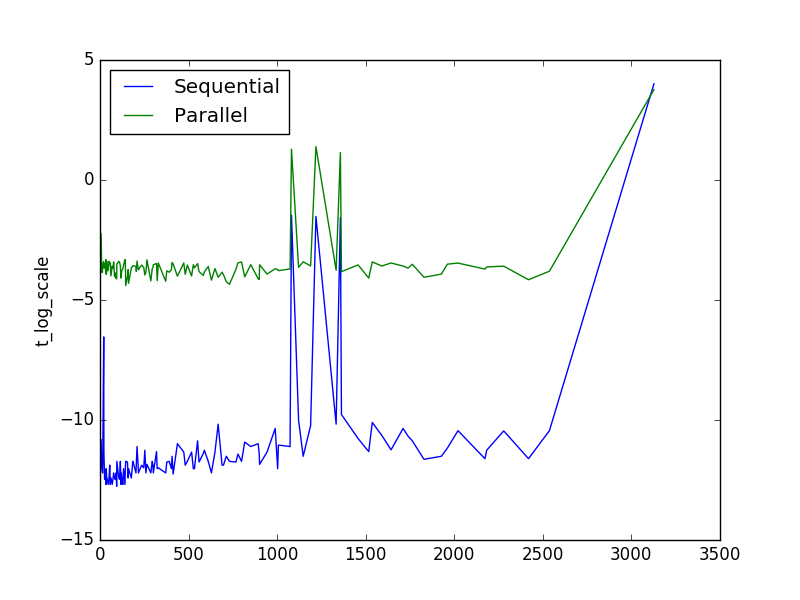
\includegraphics[width=0.7\textwidth]{figure_1.png}
\end{figure}\\
we can clearly see the presence of overheads when numbers are small, and the advantage of paralelization can be realized when $N$ is large, e.g. $N=53\times59$ \\
\begin{figure}[h!]
	\centering
	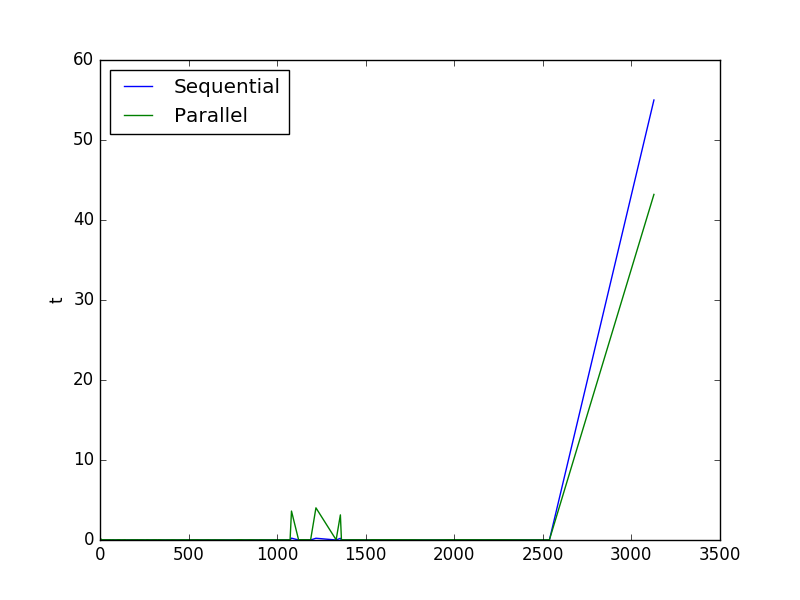
\includegraphics[width=0.7\textwidth]{figure_2.png}
\end{figure} \\
So we see how parallelism can be used to accelerate the prime factor, and if the parallel is done on a GPU we could certainly expect a even shorter running time. In the following section, we will introduce a different prime factor technique called Pollard Rho, and from that we shall illustrate a point when applying parallelization that sometimes it may not be important how well the parallel program is written, but how efficient the base case -- sequential implementation is.

\section{Pollard Rho}
...


























\newpage
\section*{Appendix A.1}
\begin{verbatim}
# load library
import numpy as np
import sys
import time
from fractions import gcd

#Define sequential implementation of pollard p-1
def pollard_pm1(n):
    t1 = time.time()
# now we find the coprime a
a = 2
while gcd(a, n) != 1:
    a += 1
t2 = time.time()
print "Finding a took: %.10f sec" % (t2 - t1)
print "Coprime a is: ", a
# now look for prime factors
def prime_factor(k):
    L = np.math.factorial(k)
return gcd(a**L-1, n)
k = 1
result = 1
while result in [1, n]:
    result = prime_factor(k)
    k += 1
t3 = time.time()
print "Total time used %.16f sec" % (t3 - t1)
if result in [1, n]:
    print "Current iteration did not find prime facotr of N! or N is prime"
else:
    print "Prime factors are %d ad %d" % (result, n/result)

# use small prime numbers for p-1: https://primes.utm.edu/lists/small/1000.txt
N = 53*59
pollard_pm1(N)
\end{verbatim}
\section*{Appendix A.2}
\begin{verbatim}
# load library
import numpy as np
import sys
import time
from fractions import gcd
from multiprocessing import Pool

n = 53*59
t1 = time.time()
# now we find the coprime a
a = 2
while gcd(a, n) != 1:
    a += 1
t2 = time.time()
print "Finding a took: %.10f sec" % (t2 - t1)
print "Coprime a is: ", a
# now look for prime factors
def prime_factor(k):
    L = np.math.factorial(k)
return gcd(a**L-1, n)
k = 2
result = 1
p = Pool(4) # use Pool from multiprocessing, use 4 processors
while result in [1, n]:
    results = p.map(prime_factor, [k, k+1, k+2, k+3])
    k += 4
for i in results:
    if i not in [1, n]:
        result = i
t3 = time.time()
p.close()
p.join()
print "Total time used %.16f sec" % (t3 - t1)
if result in [1, n]:
print "Current iteration did not find prime facotr of N! or N is prime"
else:
print "Prime factors are %d ad %d" % (result, n/result)
\end{verbatim}


\newpage
\begin{thebibliography}{9}
	\bibitem{fermat} 
	\textit{Fermat's little theorem},\\
	\url{https://en.wikipedia.org/wiki/Fermat's_little_theorem}
	
	\bibitem{suzuki}
	\textit{pollards p 1 factorization}, Jeff Suzuki, Brooklyn College\\
	\url{https://www.youtube.com/watch?v=fFJMoIj71nQ}
\end{thebibliography}
\end{document}